\documentclass[11pt,letterpaper]{article}
\usepackage[top=1.00in, bottom=1.0in, left=1in, right=1.25in]{geometry}
\usepackage{graphicx}
\usepackage{latexsym,amssymb,epsf}
\usepackage{epstopdf}

\usepackage{sectsty,setspace,natbib}
\usepackage{float}
\usepackage{latexsym}
\usepackage{epsfig}
\usepackage{graphicx}
\usepackage{amsmath}
\usepackage{array}
\usepackage{lineno}
\usepackage{gensymb}
\usepackage{xr-hyper}
\externaldocument{phencc_supp}
% \usepackage{hyperref}

\usepackage{framed}

\linespread{1.1} % was 1.66 for double-spaced 
% \raggedright
\setlength{\parindent}{0.5in}
\pagestyle{empty}

\parskip=5pt
\pagenumbering{arabic}
\pagestyle{plain}
\setlength\parindent{0pt}

\begin{document}
\begin{flushright}
Version dated: \today
\end{flushright}
\bigskip
\noindent Running title: Environmental tracking 
% put in your own RH (running head)
\bigskip
\medskip
\begin{center}
% Insert your title:
\noindent{\Large {\bf How environmental tracking shapes communities in \\ stationary \& non-stationary systems}}\\
% Other titles: `Environmental tracking: It's more complicated than you think' (we hope) 
% or `Environmental tracking: Is it naive? Or, are we just naive?'
\bigskip
\noindent {\normalsize
E. M. Wolkovich$^{1}$ \& M. J. Donahue$^{2}$ }\\
\noindent {\small \it
$^1$ Forest \& Conservation Sciences, Faculty of Forestry, University of British Columbia, 2424 Main Mall, Vancouver, BC V6T 1Z4 (e.wolkovich@ubc.ca)\\
$^2$ Hawaii Institute of Marine Biology, University of Hawai`i at M\= anoa, K\=an`eohe, HI 96744 (donahuem@hawaii.edu)}\\
\medskip
\end{center}
\noindent{\bf Corresponding author:} see$^{1}$ above; Ph: 604.827.5246 (no fax).\\

\noindent \emph{Authorship statement:} EMW and MJD both conceived of the paper, performed modeling work and edited the paper, EMW additionally wrote the paper and did the literature review, while MJD additionally wrote the supplementary information on the model.  \\
\noindent \emph{Data statement:} Review, so no new primary data, but data from a comprehensive literature review will be archived in an appropriate public repository and the data DOI will be included at the end of the article. \\
\noindent \emph{Keywords:} community assembly, global change, climate change, phenology, environmental variability\\
\noindent \emph{Article type:} Reviews and Syntheses\\
\noindent \emph{Article information:} Abstract: 196 words; Main text: 5830; Figures: 4; Boxes: 3 (text in Box 1: 690; Box 2: 385; Box 3: 264); 93 references
% main text words (5500 without in-text refs approximately) 
\newpage
% \linenumbers % If you want to add need to add \begin{linenomath} and \end{linenomath} around all eqns (and check they still show up)

\begin{abstract} 
The modeling paper ... 
\end{abstract}

\newpage
\section{Main text} % Lizzie tried to only put text here that we did NOT use in the main text or supp of the (now primarily) review paper.




In the model, the population census of seeds, $N$, occurs at time $t$ at the end of the growing season (Equation 1).  Seeds survive over winter at rate $s$ and are lost from the population at rate $(1-s)$.  Surviving seeds germinate at rate $g_{i}(t)$.  Seeds that do not germinate remain in the seed bank until the next census at $t+1$.  Germination rate is a Gaussian function that declines with the distance between $\tau_{i}$, the species-specific preferred germination time, and $\tau_{p}(t)$, the timing of the resource pulse in year $t$, with maximum germination when $\tau_{i} = \tau_{p}(t)$ (Equation 6, Fig. \ref{fig:concept}a,b).  In cases that include tracking, the distance between $\tau_{i}$ and  $\tau_{p(t)}$ can be reduced by tracking, $\alpha_{i}$, resulting in greater germination fraction (Equation 7). \\

Germinating seeds are converted to seedling biomass at rate $b_{0}$ (Equation 4). Within year dynamics of the two species follows $R^{*}$ competition for a single resource.  The growing season begins with a single resource pulse $R_0(t)$.  Both  species consume the resource at rate $f(R)$ (Equation 3), and the resource undergoes abiotic loss (e.g., evapotranspiration) at rate $\epsilon$ (Equation 5).  Differences in $R^{*}_{i}$ were generated by differences in conversion efficiency, $c_{i}$. Species were otherwise identical in resource update parameters ($a$, $u$, and $\theta$) and in metabolic loss ($m$).  Biomass at the end of the season is converted into seeds at rate $\phi$, and the population of seeds is censused at $t+1$. \\

Interannual variation occurs in both the timing and the amount of the resource pulse.  The timing of the resource pulse varies from year to year and is given by $\tau_{p}(t)$, which is drawn from a $\beta$ distribution. The amount of resource available at the beginning of each season, $R_0(t)$, varies from year to year and is drawn from a log-normal distribution.  Each model run is comprised of a 500 year stationary period and a 500 year nonstationary period.  During the stationary period, $R_0(t)$ and $\tau_{p}(t)$ are each drawn from a stationary distribution.  During the nonstationary period, the timing of the resource pulse, $\tau_{p}(t)$, gradually shifts earlier in the season (Fig. \ref{fig:fig_Rt_tauPt}).  For the model runs displayed in Fig. \ref{fig:tauirstar} and Fig. \ref{fig:alpharstar}, this shift in the timing of the resource pulse is the only change in the environment during the nonstationary period.  We also discuss model runs in which the amount of resource, $R_0(t)$,  declines during the nonstationary period along with the shift in timing, $\tau_{p}(t)$ (Fig. \ref{fig:fig_Rt_tauPt}).  \\   

\subsubsection{Tracking in stationary environments}
Species must be sufficiently matched to their environment across years to persist for any long period of time. In our modeling framework, this means species must have a germination curve such that their effective biological start time ($\hat{\tau_{i}}$) is sufficiently close to the environmental start time ($\tau_{p}$) to allow germination of new seeds before the species' seedbank is exhausted. This can happen in effectively two ways: (1) species have fixed intrinsic biological start time values ($\tau_i$) close enough to the environmental start time ($\tau_p$; e.g., species A in Fig. \ref{fig:concept}b) to persist, or (2) species have a combination of an intrinsic biological start time ($\tau_i$) and tracking ($\alpha$) that brings the species' effective biological start time ($\hat{\tau_{i}}$) close enough to the environmental start time (e.g., see species B in Fig. \ref{fig:concept}b) to persist.  

A simple outcome of this model is that in temporally variable environments where all other species characteristics are identical, the species with the effective biological start time closest to the average environmental start time will always win---regardless of whether this effective biological start is due to a fixed intrinsic start time or due to tracking (or some combination of the two). Put another way, in a stationary environment both tracking and a fixed intrinsic start time are equally useful ways to match to the environment---all that matters is the effective distance between the biological and environmental start of the season. This is because both represent the same niche axis---the temporal niche. 

% (A large chunk of this is in review paper as of 21 Feb 2020.) As both a fixed intrinsic start time and tracking represent the same major niche axis, species cannot coexist given only variation in these traits---coexistence requires variation in another trait axis. As discussed above, theory and empirical work suggest this trade-off may involve traits related closely to resource competition. With this added variation---here we varied species' $R^*$ (via $c_i$)---species can persist together as long as those species with a temporal niche advantage are also the inferior competitors (Fig. \ref{fig:tauirstar}-\ref{fig:alpharstar}). That is, species that can draw resources down to a lower level and are thus the superior within-season resource competitors (lower $R^*$) can persist with species with that are inferior competitors but have realized biological start times closer to the environmental start time (regardless of whether that realized biological start time is a result of a fixed trait or tracking)---a finding inline with currently observed empirical trade-offs (see Box `Trait trade-offs with tracking'). These trade-offs, however, are all environmentally dependent. They hold only so long as the environment is stationary. 



\subsubsection{Tracking in non-stationary environments}

The two species coexistence model (see Equations 1-6 above) includes both interannual variation in the environment and intra-annual resource competition.  The model was modified from \citet{Chesson:2004eo}, which was originally conceptualized for annual plants with a seedbank.  Although the model can be conceived of more generally, we use the language of annual plant germination for concreteness.  

In communities where species traded-off competitive traits ($R^*$) with non-trackers---species with fixed intrinsic biological start times ($\tau_i$)---species with earlier start times were clearly favored in the non-stationary environment, generally driving the other species (with a lower $R^*$ and later start time) extinct before the end of our 500 year time-period (Fig. \ref{fig:tauirstar}). Very few two-species communities persisted through the end of the non-stationary period (2 out of 547 two-species communities persisting after end of stationary, or 0.04\%); those that persisted did so because the strong similarity between the two species slowed competitive exclusion (i.e., the two species were nearly identical in both $R^*$ and intrinsic biological start time, $\tau_i$). These species were thus persisting mainly through equalizing mechanisms. In the previous stationary environment species coexisted through both equalizing and stabilizing mechanisms, but the stabilizing mechanisms were lost in the non-stationary environment, as the system shifted away from the region of the temporal niche axis that the communities formed in. 
% Very few two-species communities persisted through the end of the non-stationary period (2 out of 547 two-species communities persisting after end of stationary, or 0.04\%) and those that did were generally persisting via being highly similar---having nearly identical $R^*$ and fixed intrinsic biological start time traits ($\tau_i$). These species were persisting through equalizing mechanisms---by being almost the same neither species could drive the other extinct, though these species do not coexist (as in longer simulations one species would be lost through drift or related mechanisms). The contrast of equalizing mechanisms---stabilizing mechanisms---include niche differences, such as the trade-off in competitive traits ($R^*$) with a fixed intrinsic biological start time trait ($\tau_i$). Yet, in this non-stationary system stabilizing mechanisms failed to yield any persistence of two-species communities as the environment shifted away from the previous trade-off axis the communities formed in. 

Persistence of two-species communities via both stabilizing and equalizing mechanisms occurred more often in communities where species traded off competitive traits ($R^*$) with tracking ($\alpha$). 
...
Tracking, in contrast to fixed biological start times, allowed the species with the competitive advantage in effective start time to shift along the temporal niche axis as the environment shifted.  


\subsubsection{Model conclusions}

While in stationary systems both tracking and a fixed intrinsic start time can allow a good match to the environment, tracking is superior as environments shift to non-stationarity, confirming the current paradigm that climate change favors species that track the environment. 

Our model, however, makes a number of assumptions about how species respond to non-stationarity in the environment. We imposed environmental non-stationarity on an axis fundamental to coexistence. Yet, non-stationarity in the environment can take on many forms---both in what variable it affects and how it reshapes the underlying distribution of that variable. Communities that assemble via other axes of the environment than start of season timing may be far less impacted than our simulations suggest. Further, we examined a common trend with climate change---shifts in the mean of the environment. Changes can also occur in the variance or the fundamental shape of the distribution (e.g., shifting from a normal distribution to one that is more similar to a Gamma). Additionally, we applied a shift to only one aspect of the environment. In reality, climate change may impose multivariate shifts.

Human modification of the globe imposes complex shifts in the environments of most species. If the environment shifts along multiple niche axes involved in community assembly, it may allow trade-offs that structure communities to persist through non-stationary periods. We examined this possibility by again shifting the mean start of season earlier (i.e., changing the temporal niche) and, at the same time, decreasing the mean size of the resource pulse by half (i.e., changing the resource niche). Thus, our environment simultaneously favored species with earlier start times and superior within-season competitive abilities (lower R*). We found little evidence, however, of communities persisting via a maintained trade-off---instead the inherent variability of a system shifting in two dimensions drove species extirpations higher (14.8\% of two-species communities remaining after non-stationary). Thus, while a multivariate nonstationary environments may, in principle, maintain trade-offs, the shifts in the joint distribution would need to be so balanced that it seems unlikely. More likely appears the possibility that multivariate shifts in the environment make species more vulnerable to local extirpation \citep{sixthectinction2011,IPCC:2014sm}.


%=======================================================================
% References
%=======================================================================
\newpage
\bibliography{/Users/Lizzie/Documents/git/bibtex/LizzieMainMinimal}
\bibliographystyle{/Users/Lizzie/Documents/git/bibtex/styles/ecolett.bst}


%=======================================================================
% Tables
%=======================================================================

%\begin{center}  
%\begin{table}
%\caption{Key differences between PWR and traditional PCMs such as PGLS.}
%\begin{tabular}{ | p{4cm} | p{5.5 cm} | p{5.5 cm} |}   \hline 
%& PWR & PCMs (e.g., PGLS) \\ \hline \hline
%Major goal & Study of evolution of correlation between variables across species & Study of evolution of correlation between variables across species\\ \hline
%\emph{Assumption 1:} Nature of correlation between two or more variables & Non-stationary (changes through phylogeny in a phylogenetically conserved fashion) & Stationary (constant) throughout phylogeny (all variation is noise) \\ \hline
%\emph{Assumption 2:} Completeness of variables & Substitutes phylogeny for variables (simple or complex) not in the model that interact with variables in the model & Assumes variables in model are primary drivers of correlational relationship \\ \hline
%Inferential mode & Usually exploratory & Hypothesis testing (statistical significance)\\ \hline
%Outputs & Coefficients of regression changing through the phylogeny & p-value and single set of coefficients presumed to apply to entire phylogeny with their confidence intervals\\ \hline

%Method to avoid overfitting & Cross-validation (boot-strapped determination of optimal band-width for accurate prediciton of hold-outs) & Exact analytical model of errors and degrees of freedom\\ \hline \hline
%\end{tabular}
%\end{table}
%\end{center}

%=======================================================================
% Figures
%=======================================================================
\clearpage


\begin{figure}[t!]
\centering
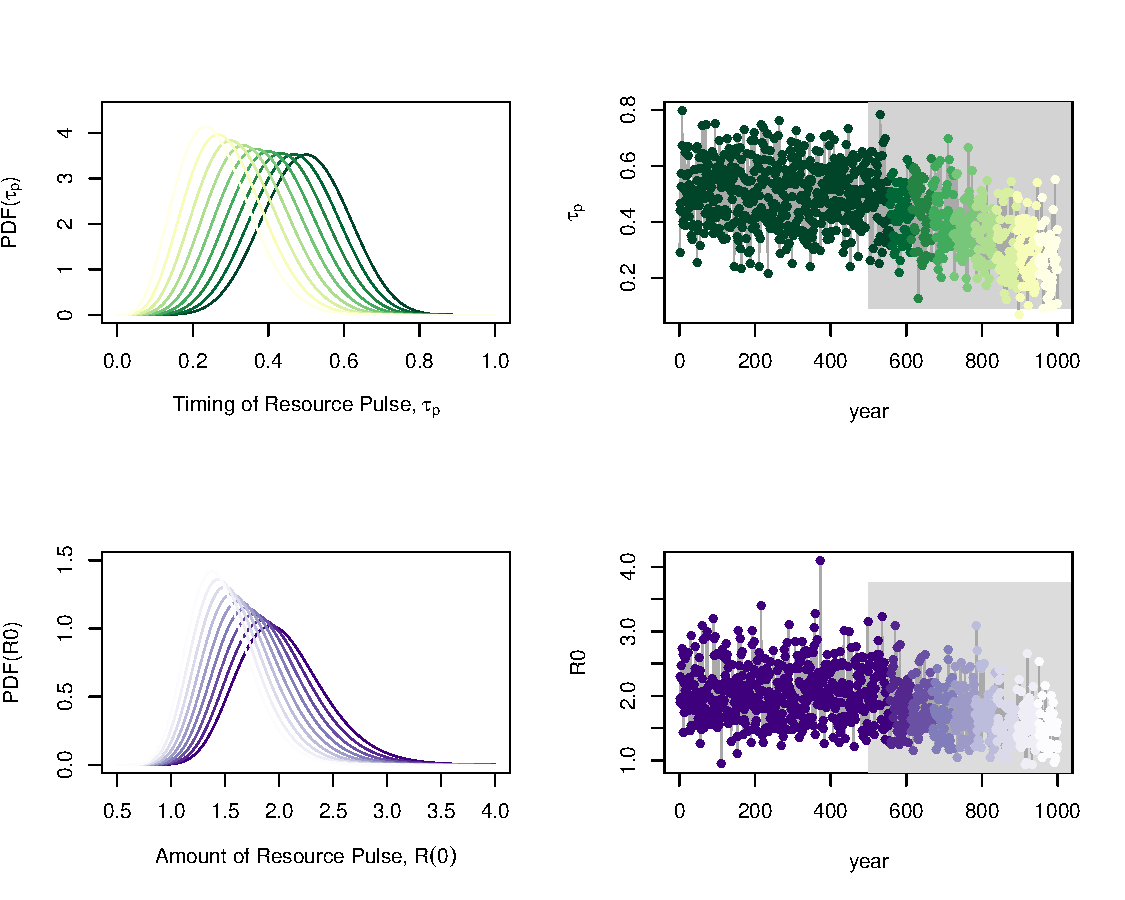
\includegraphics[width=1\textwidth]{..//..//R/graphs/modelruns/manuscript/modelsupp4panel.pdf}
\caption{How the environment shifts from the stationary period to the nonstationary period. The timing of the resource pulse shifts from $\tau_{p} \sim \beta(10,10)$ for the 500 year stationary period to $\tau_{p}$ \sim $\beta(5,15)$ over the 500 year nonstationary period.  For simulations where the amount of resource is also changing, $R(0)\sim logNormal(log(2), 2))$ during the 500 year stationary period and shifts to $R(0) \sim logNormal(log(2)/2,2)$ during the nonstationary period.}
\label{fig:fig_Rt_tauPt}
\end{figure}

\begin{figure}[t!]
\centering
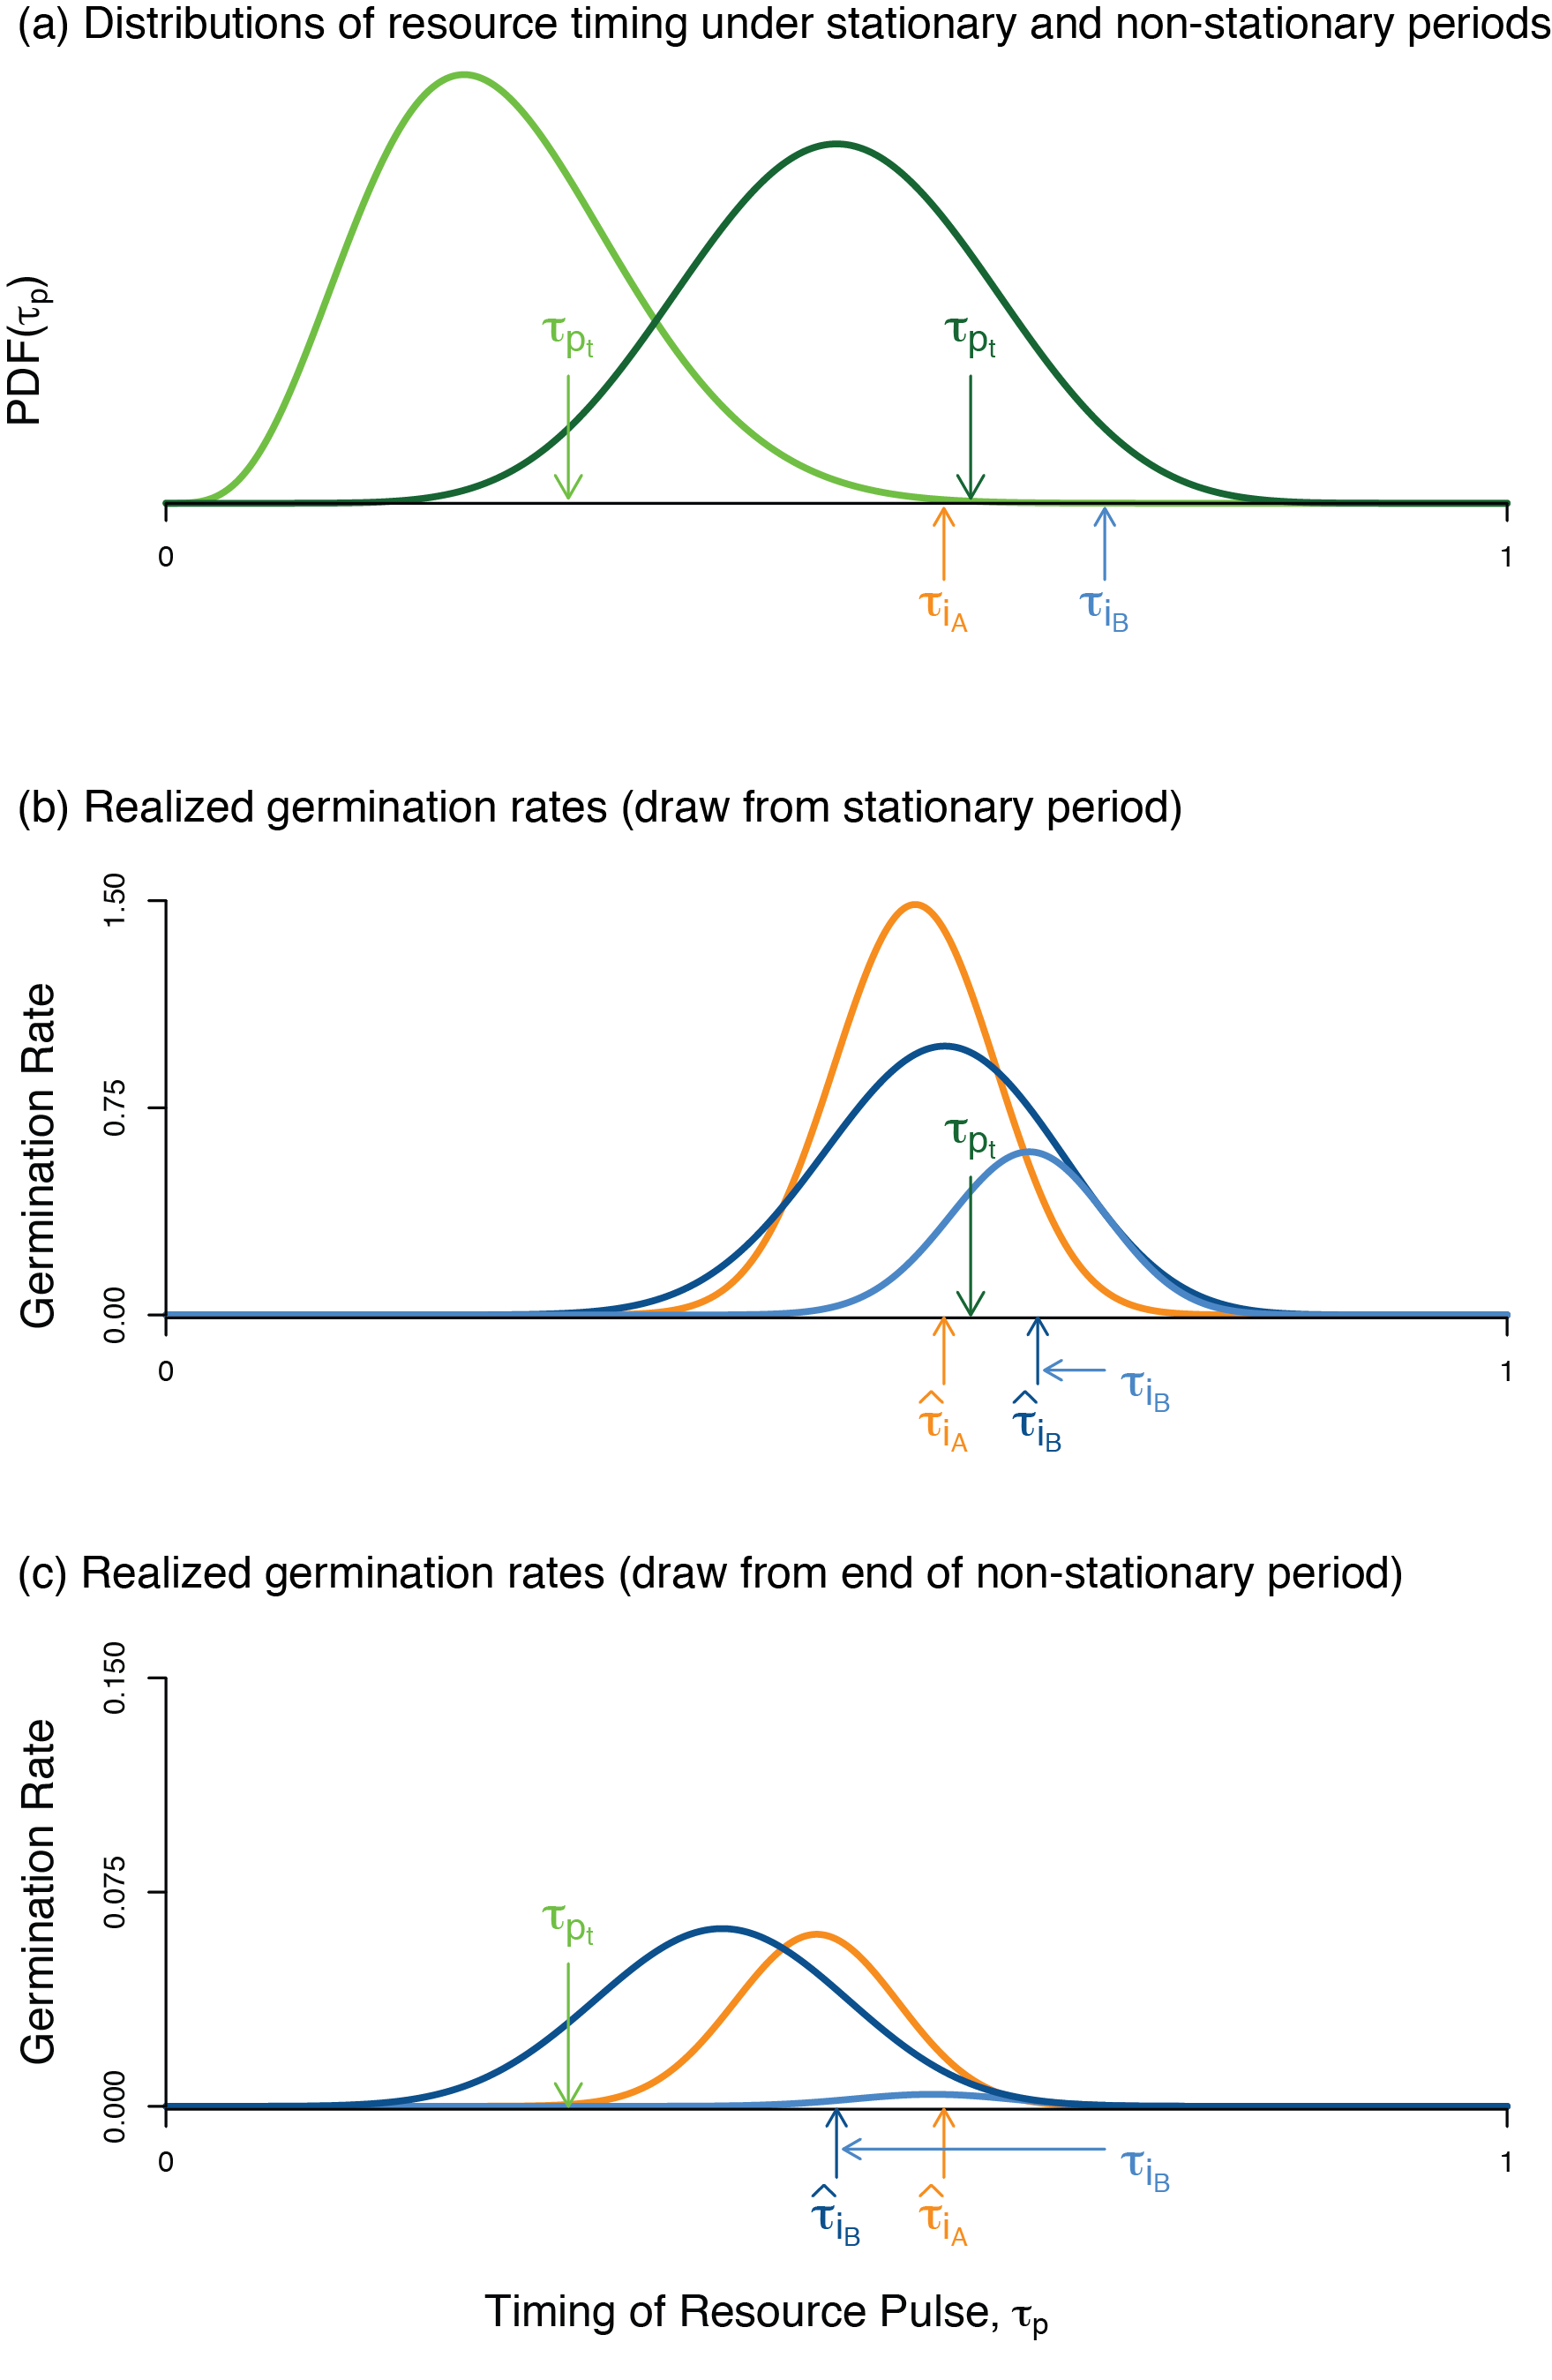
\includegraphics[width=0.65\textwidth]{..//..//R/graphs/conceptual/TauP_GerminationAdj.png} 
\caption{The distributions of the environment (a) and species' germination for two sample years (b-c) in our seed germination model. (a) The timing of the resource pulse ($\tau_p(t)$), which defines the environmental start of season, is $\beta$-distributed with parameters $\beta(10,10)$ during the stationary period (dark green) shifting to $\beta (5,15)$ through the nonstationary period (light green). (b) Realized germination rate as a function of $\tau_p(t)$ for two species during the stationary period: the orange line is a non-tracking species A with preferred germination time, $\tau_{iA}$, that is close to the mean of the stationary period; the blue lines show the difference in realized germination rate of a tracking species with a preferred germination time, $\tau_{iB}$, that is further from the mean of the stationary period both without (light blue) and with (dark blue) the effect of tracking; note the shift from $\tau_{iB}$ to $\hat{\tau_{iB}}$. (c) Realized germination rate of species A and species B at the end of the nonstationary period. Note the change in axes from (b) to (c) shows the decline in overall germination rate as the environment moves away from the preferred germination time of both species.} % I'm not sure that "realized germiantion" is the best phrase, but it is the germination rate given tauP times the prob of tauP under that STA or NST period.  So it it he realized germination rate for each species given the environment.  
% If, in a particular year, $\tau_i$ is close to $\tau_p$, a large fraction of species $i$ seeds will germinate (e.g., Fig. \ref{fig:concept}b) ; if $\tau_i$ is far from $\tau_p$, a small fraction of the seeds will germinate.  Figure \ref{fig:concept} b-c illustrate the germination rate of two species with different $\tau_i$ values under two different environments.   

\label{fig:concept}
\end{figure}
%% Figure reference to the supplement isn't working in the caption for Figure 3 or 4!
\begin{figure}[t!]
\centering
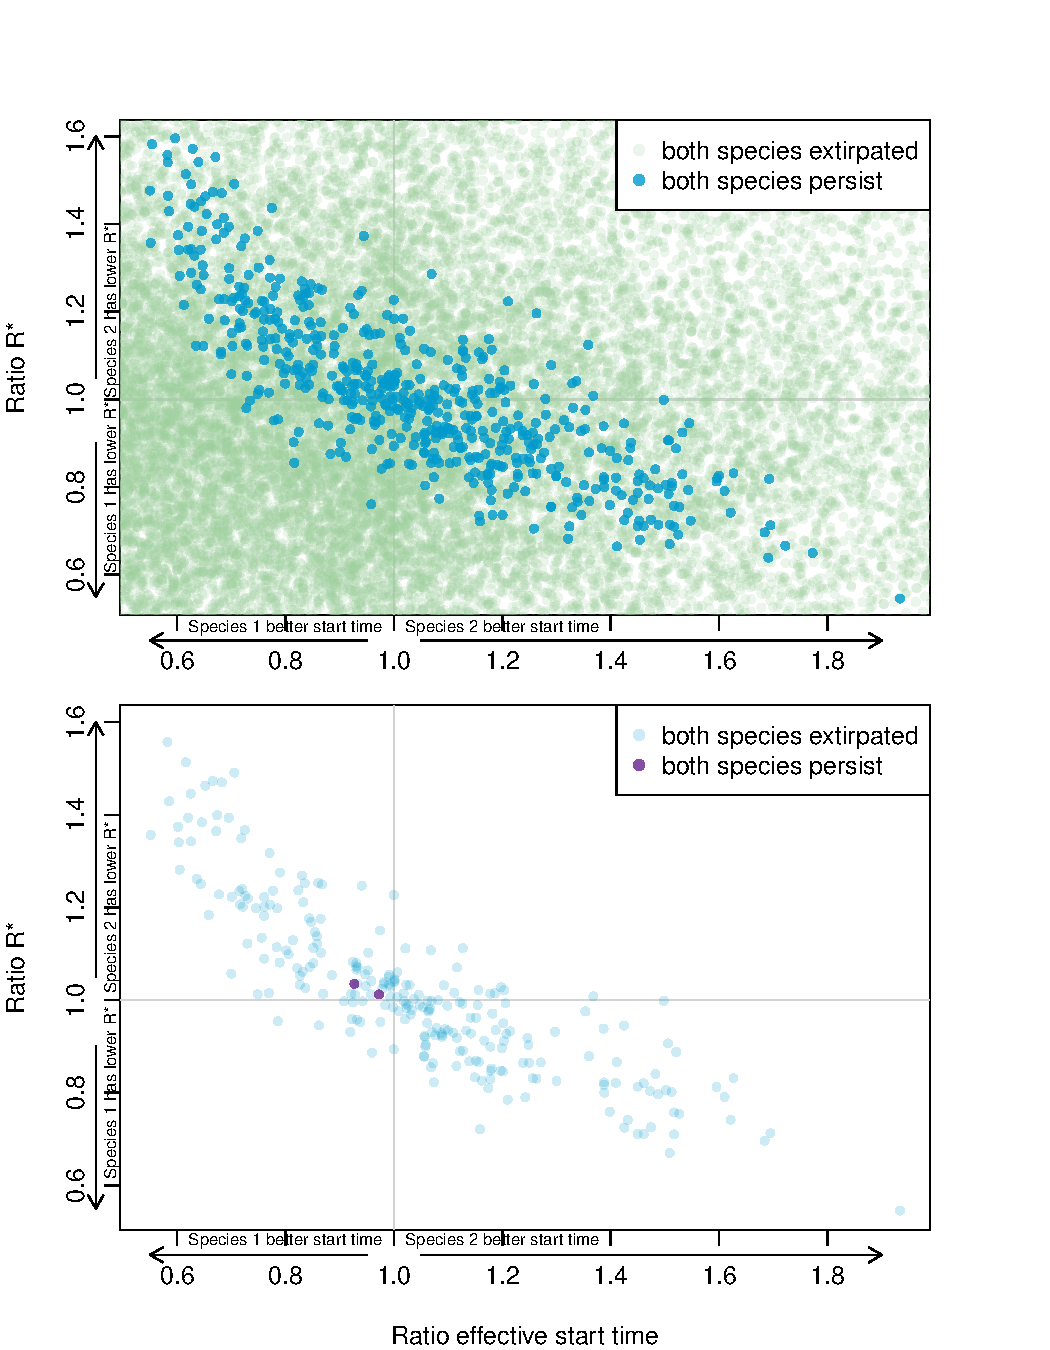
\includegraphics[width=0.9\textwidth]{..//..//R/graphs/modelruns/manuscript/tauIPrstart1_2panel.pdf}
\caption{How non-stationarity reshapes two-species communities in a simple model where effective start time (X axis: species 1/species 2) trades off with $R^*$ (Y axis: species 1/species 2): each point represents one two-species community color-coded by whether both species persisted or one or more species was extirpated through 500 years of a stationary environment (top), followed by an additional 500 years of non-stationary environment (bottom), where the abiotic start of the season shifts earlier. Only two-species communities that persisted through the stationary period are shown in the bottom panel. See Fig. \ref{fig:tauirstarsupp} for an alternative version of this figure detailing one-species outcomes.}
 \label{fig:tauirstar}
\end{figure}


\end{document}
%%%%%%%%%%%%%%%%%%%%%%%%%%%%%%%%%%%%%%%%%%%%%%%%%%%%%%%%%%%%%%%%%%%%%%%%
